\documentclass[10pt]{jsarticle}

\pagestyle{empty}

\usepackage[left=0.5cm, top=0.5cm, right=0.5cm, bottom=0.5cm, nohead, dvipdfm]{geometry}
\usepackage{comment}
\usepackage{bussproofs}
\usepackage{amsmath}
\usepackage{amssymb}
\usepackage{latexsym}
\usepackage{txfonts}
\usepackage[dvipdfmx]{graphicx}
\usepackage{tikz}
\usepackage{array}

\EnableBpAbbreviations
\newenvironment{bprooftree}
               {\leavevmode\hbox\bgroup}
               {\DisplayProof\egroup}

\usetikzlibrary{decorations.markings, shapes}
\tikzset{middlearrow/.style n args={3}{
    decoration={
      markings,
      mark=at position 0.5 with {\arrow{#1}, \node[#2]{#3};},
    },
    postaction={decorate}
  }
}

\newcommand*{\vcenteredhbox}[1]{\begingroup
\setbox0=\hbox{#1}\parbox{\wd0}{\box0}\endgroup}


\begin{document}
\begin{prooftree}
  \AxiomC{}
  \RightLabel{Id}
  \UnaryInfC{$v:\tau \vdash v:\tau$}
\end{prooftree}

\begin{prooftree}
  \AxiomC{$\Gamma \vdash \Delta$}
  \AxiomC{$\Gamma' \vdash \Delta'$}
  \RightLabel{Mix}
  \BinaryInfC{$\Gamma,\Gamma' \vdash \Delta,\Delta'$}
\end{prooftree}

\begin{prooftree}
  \AxiomC{$\Delta \vdash \Gamma$}
  \RightLabel{Flip}
  \UnaryInfC{$\Gamma \vdash \Delta$}
\end{prooftree}

\begin{center}
  \begin{bprooftree}
    \AxiomC{$\Gamma,v':\tau',v:\tau,\Gamma' \vdash \Delta$}
    \LeftLabel{Ex${}_\text{L}$}
    \UnaryInfC{$\Gamma,v:\tau,v':\tau',\Gamma' \vdash \Delta$}
  \end{bprooftree}
  \quad
  \begin{bprooftree}
    \AxiomC{$\Gamma \vdash \Delta,v':\tau',v:\tau,\Delta'$}
    \RightLabel{Ex${}_\text{R}$}
    \UnaryInfC{$\Gamma \vdash \Delta,v:\tau,v':\tau',\Delta'$}
  \end{bprooftree}
\end{center}

\begin{center}
  \begin{bprooftree}
    \AxiomC{$\Gamma \vdash v:\tau,\Delta$}
    \LeftLabel{$\star_\text{L}$}
    \UnaryInfC{$\Gamma,\langle\rangle/v:\tau^\star \vdash \Delta$}
  \end{bprooftree}
  \quad
  \begin{bprooftree}
    \AxiomC{$\Gamma,v:\tau \vdash \Delta$}
    \RightLabel{$\star_\text{R}$}
    \UnaryInfC{$\Gamma \vdash \langle\rangle/v:\tau^\star,\Delta$}
  \end{bprooftree}
\end{center}

\begin{center}
  \begin{bprooftree}
    \AxiomC{$\Gamma \vdash \Delta$}
    \LeftLabel{$\iota_\text{L}$}
    \UnaryInfC{$\Gamma,\langle\rangle:\iota \vdash \Delta$}
  \end{bprooftree}
  \quad
  \begin{bprooftree}
    \AxiomC{$\Gamma \vdash \Delta$}
    \RightLabel{$\iota_\text{R}$}
    \UnaryInfC{$\Gamma \vdash \langle\rangle:\iota,\Delta$}
  \end{bprooftree}
\end{center}

\begin{center}
  \begin{bprooftree}
    \AxiomC{$\Gamma,v_1:\tau_1,v_2:\tau_2 \vdash \Delta$}
    \LeftLabel{$\otimes_\text{L}$}
    \UnaryInfC{$\Gamma,\langle{v_1,v_2}\rangle:\tau_1\otimes\tau_2 \vdash \Delta$}
  \end{bprooftree}
  \quad
  \begin{bprooftree}
    \AxiomC{$\Gamma \vdash v_1:\tau_1,v_2:\tau_2,\Delta$}
    \RightLabel{$\otimes_\text{R}$}
    \UnaryInfC{$\Gamma \vdash \langle{v_1,v_2}\rangle:\tau_1\otimes\tau_2,\Delta$}
  \end{bprooftree}
\end{center}

\begin{center}
  \begin{bprooftree}
    \AxiomC{$\Gamma,v:\tau_1 \vdash \Delta$}
    \LeftLabel{$\oplus_\text{L${}_1$}$}
    \UnaryInfC{$\Gamma,\langle{\text{left}\;v}\rangle:\tau_1\oplus\tau_2 \vdash \Delta$}
  \end{bprooftree}
  \quad
  \begin{bprooftree}
    \AxiomC{$\Gamma \vdash v:\tau_1,\Delta$}
    \RightLabel{$\oplus_\text{R${}_1$}$}
    \UnaryInfC{$\Gamma \vdash \langle{\text{left}\;v}\rangle:\tau_1\oplus\tau_2,\Delta$}
  \end{bprooftree}
\end{center}

\begin{center}
  \begin{bprooftree}
    \AxiomC{$\Gamma,v:\tau_2 \vdash \Delta$}
    \LeftLabel{$\oplus_\text{L${}_2$}$}
    \UnaryInfC{$\Gamma,\langle{\text{right}\;v}\rangle:\tau_1\oplus\tau_2 \vdash \Delta$}
  \end{bprooftree}
  \quad
  \begin{bprooftree}
    \AxiomC{$\Gamma \vdash v:\tau_2,\Delta$}
    \RightLabel{$\oplus_\text{R${}_2$}$}
    \UnaryInfC{$\Gamma \vdash \langle{\text{right}\;v}\rangle:\tau_1\oplus\tau_2,\Delta$}
  \end{bprooftree}
\end{center}

\begin{center}
  \begin{bprooftree}
    \AxiomC{$\Gamma,v:\tau[\mu{x}.\tau/x] \vdash \Delta$}
    \LeftLabel{$\mu_\text{L}$}
    \UnaryInfC{$\Gamma,\langle{v}\rangle:\mu{x}.\tau \vdash \Delta$}
  \end{bprooftree}
  \quad
  \begin{bprooftree}
    \AxiomC{$\Gamma \vdash v:\tau[\mu{x}.\tau/x],\Delta$}
    \RightLabel{$\mu_\text{R}$}
    \UnaryInfC{$\Gamma \vdash \langle{v}\rangle:\mu{x}.\tau,\Delta$}
  \end{bprooftree}
\end{center}

\begin{center}
  \begin{bprooftree}
    \AxiomC{$\Xi,v:\tau;\Gamma \vdash \quad;\Theta$}
    \LeftLabel{$!_\text{L}$}
    \UnaryInfC{$\Xi;\Gamma,\{v\}:!\tau \vdash \quad;\Theta$}
  \end{bprooftree}
  \quad
  \begin{bprooftree}
    \AxiomC{$\Xi;\quad \vdash \Delta;v:\tau,\Theta$}
    \RightLabel{$!_\text{R}$}
    \UnaryInfC{$\Xi;\quad \vdash \{v\}:!\tau,\Delta;\Theta$}
  \end{bprooftree}
\end{center}

\begin{center}
  \begin{bprooftree}
    \AxiomC{$\Xi,v':\tau',v:\tau,\Xi';\Gamma \vdash \Delta;\Theta$}
    \LeftLabel{Classical-Ex${}_\text{L}$}
    \UnaryInfC{$\Xi,v:\tau,v':\tau',\Xi';\Gamma \vdash \Delta;\Theta$}
  \end{bprooftree}
  \quad
  \begin{bprooftree}
    \AxiomC{$\Xi;\Gamma \vdash \Delta;\Theta,v':\tau',v:\tau,\Theta'$}
    \RightLabel{Classical-Ex${}_\text{R}$}
    \UnaryInfC{$\Xi;\Gamma \vdash \Delta;\Theta,v:\tau,v':\tau',\Theta'$}
  \end{bprooftree}
\end{center}

\begin{center}
  \begin{bprooftree}
    \AxiomC{$\Xi;\Gamma \vdash \Delta;\Theta$}
    \LeftLabel{W${}_\text{L}$}
    \UnaryInfC{$\Xi,v:\tau;\Gamma \vdash \Delta;\Theta$}
  \end{bprooftree}
  \quad
  \begin{bprooftree}
    \AxiomC{$\Xi;\Gamma \vdash \Delta;\Theta$}
    \RightLabel{W${}_\text{R}$}
    \UnaryInfC{$\Xi;\Gamma \vdash \Delta;v:\tau,\Theta$}
  \end{bprooftree}
\end{center}

\begin{center}
  \begin{bprooftree}
    \AxiomC{$\Xi,v:\tau,v:\tau;\Gamma \vdash \Delta;\Theta$}
    \LeftLabel{C${}_\text{L}$}
    \UnaryInfC{$\Xi,v:\tau;\Gamma \vdash \Delta;\Theta$}
  \end{bprooftree}
  \quad
  \begin{bprooftree}
    \AxiomC{$\Xi;\Gamma \vdash \Delta;v:\tau,v:\tau,\Theta$}
    \RightLabel{C${}_\text{R}$}
    \UnaryInfC{$\Xi;\Gamma \vdash \Delta;v:\tau,\Theta$}
  \end{bprooftree}
\end{center}

\begin{center}
  \begin{bprooftree}
    \AxiomC{$\Xi;\Gamma,\{v_1\}:!\tau_1,v_2:\tau_2[v_1/x] \vdash \Delta;\Theta$}
    \LeftLabel{$\Sigma_\text{L}$}
    \UnaryInfC{$\Xi;\Gamma,\langle\{v_1\},v_2\rangle:\Sigma_{x:!\tau_1}\tau_2 \vdash \Delta;\Theta$}
  \end{bprooftree}
  \quad
  \begin{bprooftree}
    \AxiomC{$\Xi;\Gamma \vdash \{v_1\}:!\tau_1,v_2:\tau_2[v_1/x],\Delta;\Theta$}
    \RightLabel{$\Sigma_\text{R}$}
    \UnaryInfC{$\Xi;\Gamma \vdash \langle\{v_1\},v_2\rangle:\Sigma_{x:!\tau_1}\tau_2,\Delta;\Theta$}
  \end{bprooftree}
\end{center}

\begin{prooftree}
  \AxiomC{$\Xi \vdash \tau:\text{type}$}
  \RightLabel{$\star_\text{T}$}
  \UnaryInfC{$\Xi \vdash \tau^\star:\text{type}$}
\end{prooftree}

\begin{prooftree}
  \AxiomC{$$}
  \RightLabel{$\iota_\text{T}$}
  \UnaryInfC{$\vdash \iota:\text{type}$}
\end{prooftree}

\begin{prooftree}
  \AxiomC{$\Xi_1 \vdash \tau_1:\text{type}$}
  \AxiomC{$\Xi_2 \vdash \tau_2:\text{type}$}
  \RightLabel{$\otimes_\text{T}$}
  \BinaryInfC{$\Xi_1,\Xi_2 \vdash \tau_1\otimes\tau_2:\text{type}$}
\end{prooftree}

\begin{prooftree}
  \AxiomC{$\Xi_1 \vdash \tau_1:\text{type}$}
  \AxiomC{$\Xi_2 \vdash \tau_2:\text{type}$}
  \RightLabel{$\oplus_\text{T}$}
  \BinaryInfC{$\Xi_1,\Xi_2 \vdash \tau_1\oplus\tau_2:\text{type}$}
\end{prooftree}

\begin{prooftree}
  \AxiomC{$\Xi,x:\text{type} \vdash \tau:\text{type}$}
  \RightLabel{$\mu_\text{T}$}
  \UnaryInfC{$\Xi \vdash \mu{x}.\tau:\text{type}$}
\end{prooftree}

\begin{prooftree}
  \AxiomC{$\Xi \vdash \tau:\text{type}$}
  \RightLabel{$!_\text{T}$}
  \UnaryInfC{$\Xi \vdash !\tau:\text{type}$}
\end{prooftree}

\begin{prooftree}
  \AxiomC{$\Xi,x:\tau_1 \vdash \tau_2:\text{type}$}
  \RightLabel{$\Sigma_\text{T}$}
  \UnaryInfC{$\Xi \vdash \Sigma_{x:!\tau_1}\tau_2:\text{type}$}
\end{prooftree}

\newpage


\footnotesize
\begin{tabular}{lcc}
  Identity &
  \begin{bprooftree}
    \AxiomC{}
    \UnaryInfC{$v \quad id \quad v$}
  \end{bprooftree} &
  \vcenteredhbox{
    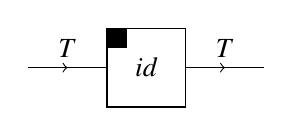
\begin{tikzpicture}
      \draw[middlearrow={>}{above}{$T$}] (0,0) -- (1,0);
      \draw (1,0.5) rectangle (2,-0.5) node[pos=.5]{$id$};
      \fill (1,0.5) rectangle (1.25,0.25);
      \draw[middlearrow={>}{above}{$T$}] (2,0) -- (3,0);
    \end{tikzpicture}
  } \\ \\
  
  Composition &
  \begin{bprooftree}
    \AxiomC{$v_1 \quad f \quad v_2$}
    \AxiomC{$v_2 \quad g \quad v_3$}
    \BinaryInfC{$v_1 \quad f;g \quad v_3$}
  \end{bprooftree} &
  \vcenteredhbox{
    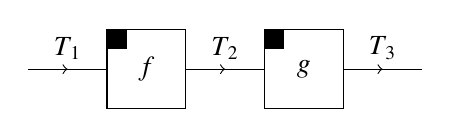
\begin{tikzpicture}
      \draw[middlearrow={>}{above}{$T_1$}] (0,0)--(1,0);
      \draw (1,0.5) rectangle (2,-0.5) node[pos=.5]{$f$};
      \fill (1,0.5) rectangle (1.25,0.25);
      \draw[middlearrow={>}{above}{$T_2$}] (2,0)--(3,0);
      \draw (3,0.5) rectangle (4,-0.5) node[pos=.5]{$g$};
      \fill (3,0.5) rectangle (3.25,0.25);
    \draw[middlearrow={>}{above}{$T_3$}] (4,0)--(5,0);
    \end{tikzpicture}
  } \\ \\

  Product &
  \begin{bprooftree}
    \AxiomC{$v_1 \quad f \quad v'_1$}
    \AxiomC{$v_2 \quad g \quad v'_2$}
    %\BinaryInfC{$\langle{v_1,v_2}\rangle \quad f\times{g} \quad \langle{v'_1,v'_2}\rangle$}
    \BinaryInfC{$(v_1*v_2) \quad f*g \quad (v'_1*v'_2)$}
  \end{bprooftree} &
  \vcenteredhbox{
    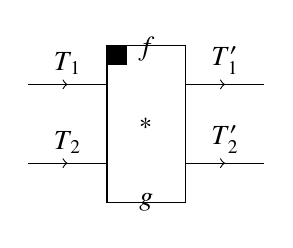
\begin{tikzpicture}
      \draw[middlearrow={>}{above}{$T_1$}] (0,0)--(1,0);
      \draw[middlearrow={>}{above}{$T_2$}] (0,-1)--(1,-1);
      \draw (1,0.5) rectangle (2,-1.5) node[pos=.5, align=center]{$f$ \\\smallskip\\ $*$ \\\smallskip\\ $g$};
      \fill (1,0.5) rectangle (1.25,0.25);
      \draw[middlearrow={>}{above}{$T'_1$}] (2,0)--(3,0);
      \draw[middlearrow={>}{above}{$T'_2$}] (2,-1)--(3,-1);
    \end{tikzpicture}
  } \\ \\

  Unitor${}_\otimes$ &
  \begin{bprooftree}
    \AxiomC{}
    \UnaryInfC{$(()*v) \quad unit_\otimes \quad v$}
  \end{bprooftree} &
  \vcenteredhbox{
    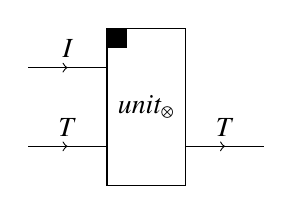
\begin{tikzpicture}
      \draw[middlearrow={>}{above}{$I$}] (0,0)--(1,0);
      \draw[middlearrow={>}{above}{$T$}] (0,-1)--(1,-1);
      \draw (1,0.5) rectangle (2,-1.5) node[pos=.5]{$unit_\otimes$};
      \fill (1,0.5) rectangle (1.25,0.25);
      \draw[middlearrow={>}{above}{$T$}] (2,-1)--(3,-1);
    \end{tikzpicture}
  } \\ \\
  
  Associator${}_\otimes$ &
  \begin{bprooftree}
    \AxiomC{}
    \UnaryInfC{$(v_1*(v_2*v_3)) \quad assoc_\otimes \quad ((v_1*v_2)*v_3)$}
  \end{bprooftree} &
  \vcenteredhbox{
    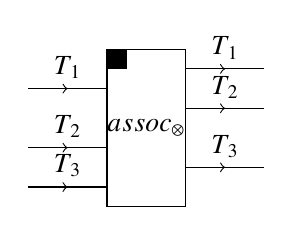
\begin{tikzpicture}
      \draw[middlearrow={>}{above}{$T_1$}] (0,0)--(1,0);
      \draw[middlearrow={>}{above}{$T_2$}] (0,-0.75)--(1,-0.75);
      \draw[middlearrow={>}{above}{$T_3$}] (0,-1.25)--(1,-1.25);
      \draw (1,0.5) rectangle (2,-1.5) node[pos=.5]{$assoc_\otimes$};
      \fill (1,0.5) rectangle (1.25,0.25);
      \draw[middlearrow={>}{above}{$T_1$}] (2,0.25)--(3,0.25);
      \draw[middlearrow={>}{above}{$T_2$}] (2,-0.25)--(3,-0.25);
      \draw[middlearrow={>}{above}{$T_3$}] (2,-1)--(3,-1);
    \end{tikzpicture}
  } \\ \\
  
  Symmetric${}_\otimes$ &
  \begin{bprooftree}
    \AxiomC{}
    \UnaryInfC{$(v_1*v_2) \quad sym_\otimes \quad (v_2*v_1)$}
  \end{bprooftree} &
  \vcenteredhbox{
    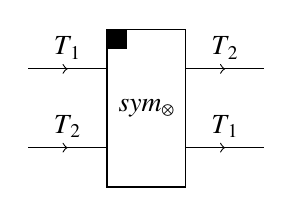
\begin{tikzpicture}
      \draw[middlearrow={>}{above}{$T_1$}] (0,0)--(1,0);
      \draw[middlearrow={>}{above}{$T_2$}] (0,-1)--(1,-1);
      \draw (1,0.5) rectangle (2,-1.5) node[pos=.5]{$sym_\otimes$};
      \fill (1,0.5) rectangle (1.25,0.25);
      \draw[middlearrow={>}{above}{$T_2$}] (2,0)--(3,0);
      \draw[middlearrow={>}{above}{$T_1$}] (2,-1)--(3,-1);
    \end{tikzpicture}
  } \\ \\
  
  Evaluation${}_\otimes$ &
  \begin{bprooftree}
    \AxiomC{}
    \UnaryInfC{$(v*()/v) \quad eval \quad ()$}
  \end{bprooftree} &
  \vcenteredhbox{
    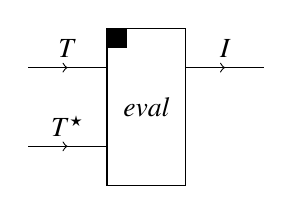
\begin{tikzpicture}
      \draw[middlearrow={>}{above}{$T$}] (0,0)--(1,0);
      \draw[middlearrow={>}{above}{$T^\star$}] (0,-1)--(1,-1);
      \draw (1,0.5) rectangle (2,-1.5) node[pos=.5]{$eval$};
      \fill (1,0.5) rectangle (1.25,0.25);
      \draw[middlearrow={>}{above}{$I$}] (2,0)--(3,0);
    \end{tikzpicture}
  } \\ \\
  
  Sum &
  \begin{tabular}{c}
    \begin{bprooftree}
      \AxiomC{$v_1 \quad f \quad v_1'$}
      \AxiomC{$v_2 \quad g \quad v_2'$}
      \BinaryInfC{$(v_1+v_2) \quad f+g \quad (v_1'+v_2')$}
    \end{bprooftree}
  \end{tabular} &
  \vcenteredhbox{
    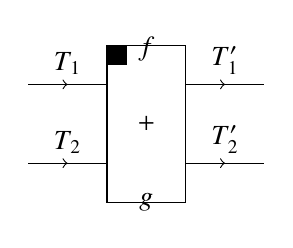
\begin{tikzpicture}
      \draw[middlearrow={>}{above}{$T_1$}] (0,0)--(1,0);
      \draw[middlearrow={>}{above}{$T_2$}] (0,-1)--(1,-1);
      \draw (1,0.5) rectangle (2,-1.5) node[pos=.5, align=center]{$f$ \\\smallskip\\ $+$ \\\smallskip\\ $g$};
      \fill (1,0.5) rectangle (1.25,0.25);
      \draw[middlearrow={>}{above}{$T'_1$}] (2,0)--(3,0);
      \draw[middlearrow={>}{above}{$T'_2$}] (2,-1)--(3,-1);
    \end{tikzpicture}
  } \\ \\

  Associator${}_\oplus$ &
  \begin{tabular}{c}
    \begin{bprooftree}
      \AxiomC{}
      \UnaryInfC{$(v_1+(v_2+v_3)) \quad assoc_\otimes \quad ((v_1+v_2)+v_3)$}
    \end{bprooftree}
  \end{tabular} &
  \vcenteredhbox{
    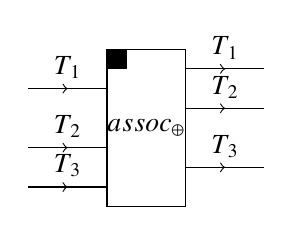
\begin{tikzpicture}
      \draw[middlearrow={>}{above}{$T_1$}] (0,0)--(1,0);
      \draw[middlearrow={>}{above}{$T_2$}] (0,-0.75)--(1,-0.75);
      \draw[middlearrow={>}{above}{$T_3$}] (0,-1.25)--(1,-1.25);
      \draw (1,0.5) rectangle (2,-1.5) node[pos=.5]{$assoc_\oplus$};
      \fill (1,0.5) rectangle (1.25,0.25);
      \draw[middlearrow={>}{above}{$T_1$}] (2,0.25)--(3,0.25);
      \draw[middlearrow={>}{above}{$T_2$}] (2,-0.25)--(3,-0.25);
      \draw[middlearrow={>}{above}{$T_3$}] (2,-1)--(3,-1);
    \end{tikzpicture}
  } \\ \\
  
  Symmetric${}_\oplus$ &
  \begin{tabular}{c}
    \begin{bprooftree}
      \AxiomC{}
      \UnaryInfC{$(v_1+v_2) \quad sym_\oplus \quad (v_1+v_2)$}
    \end{bprooftree}
  \end{tabular} &
  \vcenteredhbox{
    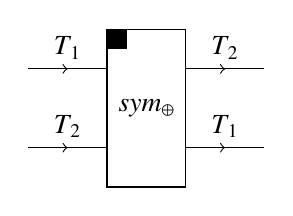
\begin{tikzpicture}
      \draw[middlearrow={>}{above}{$T_1$}] (0,0)--(1,0);
      \draw[middlearrow={>}{above}{$T_2$}] (0,-1)--(1,-1);
      \draw (1,0.5) rectangle (2,-1.5) node[pos=.5]{$sym_\oplus$};
      \fill (1,0.5) rectangle (1.25,0.25);
      \draw[middlearrow={>}{above}{$T_2$}] (2,0)--(3,0);
      \draw[middlearrow={>}{above}{$T_1$}] (2,-1)--(3,-1);
    \end{tikzpicture}
  } \\ \\

  Distribution &
  \begin{tabular}{c}
    \begin{bprooftree}
      \AxiomC{}
      \UnaryInfC{$((v_1+v_2)*v_3) \quad distrib \quad ((v_1*v_3)+(v_2*v_3))$}
    \end{bprooftree}
  \end{tabular} &
  \vcenteredhbox{
    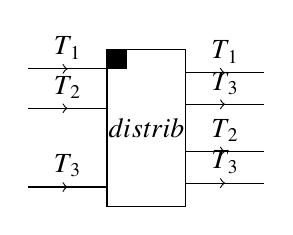
\begin{tikzpicture}
      \draw[middlearrow={>}{above}{$T_1$}] (0,0.25)--(1,0.25);
      \draw[middlearrow={>}{above}{$T_2$}] (0,-0.25)--(1,-0.25);
      \draw[middlearrow={>}{above}{$T_3$}] (0,-1.25)--(1,-1.25);
      \draw (1,0.5) rectangle (2,-1.5) node[pos=.5]{$distrib$};
      \fill (1,0.5) rectangle (1.25,0.25);
      \draw[middlearrow={>}{above}{$T_1$}] (2,0.2)--(3,0.2);
      \draw[middlearrow={>}{above}{$T_3$}] (2,-0.2)--(3,-0.2);
      \draw[middlearrow={>}{above}{$T_2$}] (2,-0.8)--(3,-0.8);
      \draw[middlearrow={>}{above}{$T_3$}] (2,-1.2)--(3,-1.2);
    \end{tikzpicture}
  } \\ \\
  
  Fold &
  \begin{bprooftree}
    \AxiomC{}
    \UnaryInfC{$\langle{v}\rangle \quad fold \quad v$}
  \end{bprooftree} &
  \vcenteredhbox{
    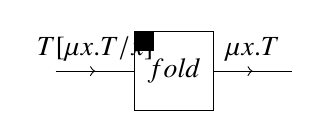
\begin{tikzpicture}
      \draw[middlearrow={>}{above}{$T[\mu{x}.T/x]$}] (0,0) -- (1,0);
      \draw (1,0.5) rectangle (2,-0.5) node[pos=.5]{$fold$};
      \fill (1,0.5) rectangle (1.25,0.25);
      \draw[middlearrow={>}{above}{$\mu{x}.T$}] (2,0) -- (3,0);
    \end{tikzpicture}
  }
\end{tabular}
\end{document}
